\begin{figure}[htb]
     \centering
     \begin{subfigure}[b]{0.3\textwidth}
      \centering
         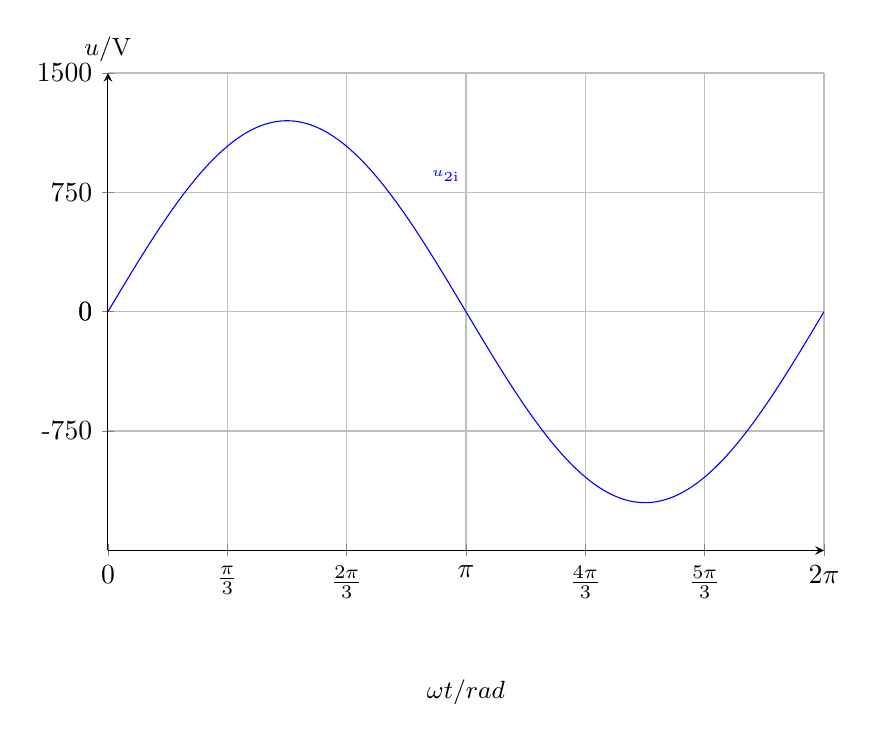
\begin{tikzpicture}
              \pgfplotsset{set layers}
         \begin{axis}[
          % x/y range adjustment
          scale only axis,
          ymin=-1500, ymax=1500,
          xmin=0, xmax=360,
%          axis x line=none, 
          samples=500,
          axis y line=center,
          axis x line=bottom,
          extra y ticks=0,
          % Label text
          xlabel={\small$\omega t / \text{rad}$},
          ylabel={\small$u/\mathrm{V}$},
          % Label adjustment
          x label style={at={(axis description cs:0.5,-0.25)},anchor=north},
          y label style={at={(axis description cs:0,.97)},anchor=south,yshift=0.2cm},
          width=0.75\textwidth,
          height=0.5\textwidth,
          % x-Ticks
          xtick={0,60,120,180,240, 300, 360},
          xticklabels={0,$\frac{\pi}{3}$,$\frac{2\pi}{3}$,$\pi$,$\frac{4\pi}{3}$, $\frac{5\pi}{3}$, $2\pi$},
          xticklabel style = {anchor=north},
          % y-Ticks
          ytick={-1500,-750,0,750,1500},
          yticklabels={-1500,-750,0,750,1500},
          yticklabel style = {anchor=east},
          % Grid layout
          grid,
          %grid style={line width=.1pt, draw=gray!10},
          %major grid style={line width=.2pt,draw=gray!90},
      ] 
      % signal u_i
      \addplot[blue, domain= 0:360, solid] {1200*sin(x)};
      % Label of u_2i
      \node[blue, fill=white, inner sep = 1pt, anchor = south] at (axis cs:170,800) {\tiny$u_\mathrm{2i}$};
         \end{axis}
         \end{tikzpicture}
         \caption{Starting}
         \label{fig:time:Starting}
     \end{subfigure}
     \hfill
     \begin{subfigure}[b]{0.3\textwidth}
        \centering
         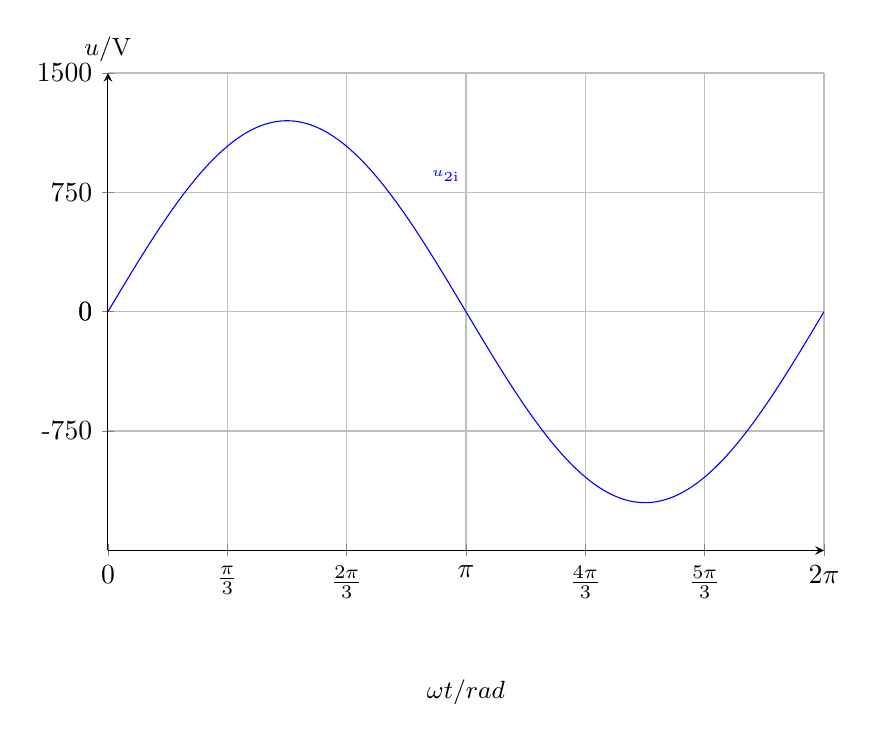
\begin{tikzpicture}
              \pgfplotsset{set layers}
         \begin{axis}[
          % x/y range adjustment
          scale only axis,
          ymin=-1500, ymax=1500,
          xmin=0, xmax=360,
%          axis x line=none, 
          samples=500,
          axis y line=center,
          axis x line=bottom,
          extra y ticks=0,
          % Label text
          xlabel={\small$\omega t / \text{rad}$},
          ylabel={\small$u/\mathrm{V}$},
          % Label adjustment
          x label style={at={(axis description cs:0.5,-0.25)},anchor=north},
          y label style={at={(axis description cs:0,.97)},anchor=south,yshift=0.2cm},
          width=0.75\textwidth,
          height=0.5\textwidth,
          % x-Ticks
          xtick={0,60,120,180,240, 300, 360},
          xticklabels={0,$\frac{\pi}{3}$,$\frac{2\pi}{3}$,$\pi$,$\frac{4\pi}{3}$, $\frac{5\pi}{3}$, $2\pi$},
          xticklabel style = {anchor=north},
          % y-Ticks
          ytick={-1500,-750,0,750,1500},
          yticklabels={-1500,-750,0,750,1500},
          yticklabel style = {anchor=east},
          % Grid layout
          grid,
          %grid style={line width=.1pt, draw=gray!10},
          %major grid style={line width=.2pt,draw=gray!90},
      ] 
      % signal u_i
      \addplot[blue, domain= 0:360, solid] {1200*sin(x)};
           % Label of u_2i
      \node[blue, fill=white, inner sep = 1pt, anchor = south] at (axis cs:170,800) {\tiny$u_\mathrm{2i}$};
         \end{axis}
         \end{tikzpicture}
         \caption{Rolling}
         \label{fig:time:Rolling}
     \end{subfigure}
     \hfill
     \begin{subfigure}[b]{0.3\textwidth}
         \centering
         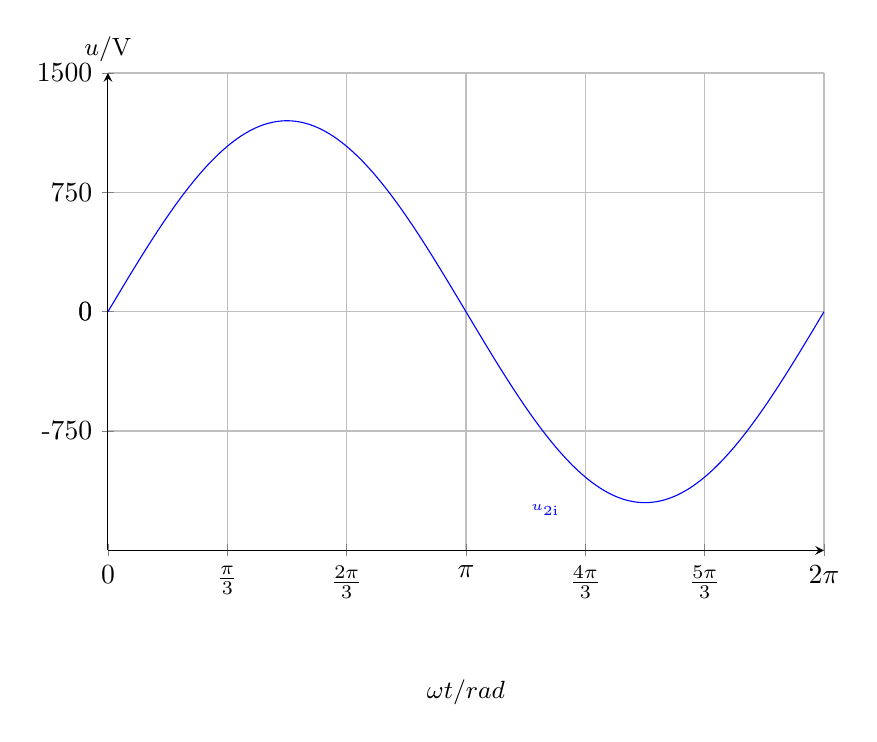
\begin{tikzpicture}
              \pgfplotsset{set layers}
         \begin{axis}[
          % x/y range adjustment
          scale only axis,
          ymin=-1500, ymax=1500,
          xmin=0, xmax=360,
   %       axis x line=none, 
          samples=500,
          axis y line=center,
          axis x line=bottom,
          extra y ticks=0,
          % Label text
          xlabel={\small$\omega t / \text{rad}$},
          ylabel={\small$u/\mathrm{V}$},
          % Label adjustment
          x label style={at={(axis description cs:0.5,-0.25)},anchor=north},
          y label style={at={(axis description cs:0,.97)},anchor=south,yshift=0.2cm},
          width=0.75\textwidth,
          height=0.5\textwidth,
          % x-Ticks
          xtick={0,60,120,180,240, 300, 360},
          xticklabels={0,$\frac{\pi}{3}$,$\frac{2\pi}{3}$,$\pi$,$\frac{4\pi}{3}$, $\frac{5\pi}{3}$, $2\pi$},
          xticklabel style = {anchor=north},
          % y-Ticks
          ytick={-1500,-750,0,750,1500},
          yticklabels={-1500,-750,0,750,1500},
          yticklabel style = {anchor=east},
          % Grid layout
          grid,
          %grid style={line width=.1pt, draw=gray!10},
          %major grid style={line width=.2pt,draw=gray!90},
      ] 
      % signal u_i
      \addplot[blue, domain= 0:360, solid] {1200*sin(x)};
           % Label of u_2i
      \node[blue, fill=white, inner sep = 1pt, anchor = south] at (axis cs:220,-1300) {\tiny$u_\mathrm{2i}$};
         \end{axis}
         \end{tikzpicture}
         \caption{Braking}
         \label{fig:time:Braking}
     \end{subfigure}
        \caption{Signals $u^\mathrm{(1)}_\mathrm{2}(t)$,
$u^\mathrm{(1)}_\mathrm{L}(t)$, $i^\mathrm{(1)}_\mathrm{2}(t)$ in different operating modes.}
        \label{fig:subtask4.1_time}
\end{figure}